%&pdflatex
\documentclass[11pt]{article}

\usepackage{geometry}                % See geometry.pdf to learn the layout options. There are lots.
\geometry{letterpaper}                   % ... or a4paper or a5paper or ...
\usepackage{graphicx}
\usepackage{longtable}

\setlength{\parindent}{0pt}
\setlength{\parskip}{\baselineskip}%

\title{Programming Practice (PRP), Coursework Exercise 4 (40\%, 40 marks)}
%\author{Martin Chapman (martin.chapman@kcl.ac.uk)}
\date{}                                           % Activate to display a given date or no date

\begin{document}
\maketitle
%\section{}
%\subsection{}

\textbf{Please read the document marked `Continuous Assessment Guidelines' carefully, before attempting any piece of coursework.}

\emph{This assignment counts for 40\% of your mark for PRP continuous assessment, and is the fourth of four. If you have not yet completed the first three assignments for PRP,  your opportunity to receive a mark for these assignments has passed. However, you are still advised to look over these assignments, and their respective model answers, before proceeding with this one.}

\emph{The release week for this assignment starts 28th November, at 23:55, and ends 5th December, at 23:55. All submissions must occur before the end of the release week.}

\textbf{This assignment is split into two problems. Problem A is a modelling task. Problem B uses this model to solve a potentially challenging problem. Students who just complete Problem A will receive a maximum grade of 70\%. Students who complete both Problems A and B can receive up to 100\%. Problem B is further subdivided into different grade boundaries. Both problems can be solved using the same set of classes. }

\textbf{It is recommended that you spend the majority of your week working on Problem A.}

\emph{If you have any questions about the structure of this assessment, please email \\ martin.chapman@kcl.ac.uk.}

\section{Problem A (70\% maximum)}

\subsection{Problem}

We want to build a simple model of a wireless network. To do this, we need to model the components involved and implement a simple protocol, the use of which will allow two components to connect. This type of protocol is known as a \emph{handshake}. Then, we want setup our network, before finally running it. 

\subsubsection{The components involved}

Wireless communication involves the following components: 
	
\begin{enumerate}
	
	\item Wireless communication occurs between \emph{network devices}. All \texttt{NetworkDevice}s have an \texttt{address}, which identifies the device.
	
	\item A \texttt{Client} (e.g. a laptop or a smartphone) and an \texttt{AccessPoint} (e.g. a home router) are special types of \texttt{NetworkDevice}. A client connects to an access point in order to use a service (e.g. to gain access to the Internet) provided by the access point.  A \texttt{Client} keeps a record of which \texttt{AccessPoint} it is currently connected to, if any. An \texttt{AccessPoint} keeps a record of the \texttt{Client}s that are \texttt{authorised} to use its services.
	
	\item Data is exchanged between network devices in the form of digital \emph{packets}. We can imagine a packet as a (postal) letter, where each \texttt{Packet} has a \texttt{destinationAddress} (to which device the letter should be sent) and a \texttt{sourceAddress} (which device sent the letter). For an example of this, see Figure 1. We will ignore the data content in a packet for the purposes of this assignment.
	
	\item  Network devices do not exchange packets directly. Instead, they place packets into a channel. Multiple devices can use the same channel, and all devices read from that channel in order to locate packets addressed to them. \texttt{Channel}s  each have a \texttt{number}, and contain \texttt{traffic}, which is a record of the \texttt{Packet}s currently in the channel. 
	
	\item Each \texttt{NetworkDevice} has the ability to \texttt{join} a \texttt{Channel}, but can only exist in one \texttt{Channel} at a time.
	
	\item When an \texttt{AccessPoint} is \texttt{add}ed to a \texttt{Network}, it \texttt{joins} a new \texttt{Channel}  upon which to communicate. It should be possible to obtain a list of the \texttt{Channel}s that are in use in a \texttt{Network}. However, for security, it should \emph{not} be possible to access the \texttt{Channel} in use by a \texttt{NetworkDevice} directly. Instead, the \texttt{Network} should keep a private record of which \texttt{Channel}s are in use by different \texttt{NetworkDevices}.
		
\end{enumerate}

\begin{figure}
  	
	\centering
 		
	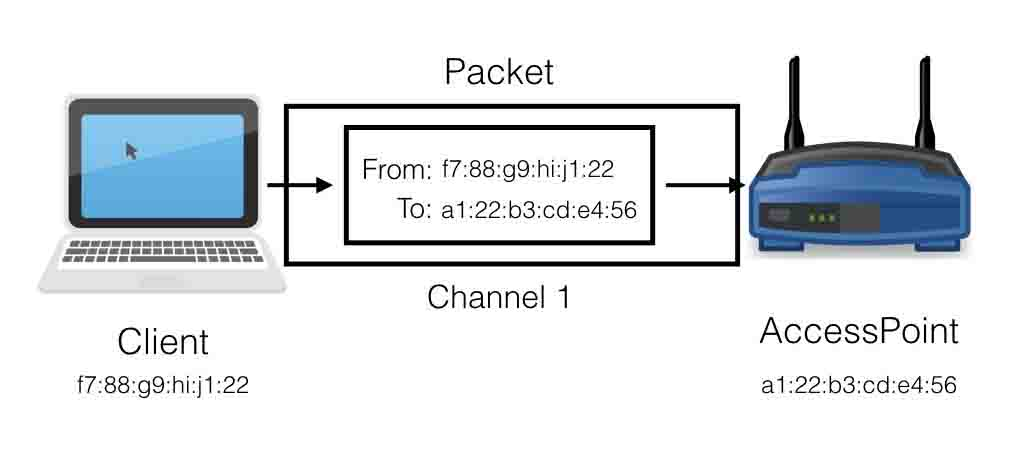
\includegraphics[width=12cm]{/Library/Server/Web/Data/Sites/webserver/PRP/distribute/CSnUsTh4/Assignment4.jpg}

	\caption{Communication between a \texttt{Client} and an \texttt{AccessPoint} (both with an address) takes place using a packet, which is a (postal) letter containing a `from' and `to' label, passed into a \texttt{Channel} that is shared by both devices.}

	\label{fig:assignment4}

\end{figure}

\subsubsection{Handshake Authentication}

	Once a network has been setup with at least one access point, and that access point has a channel, a \texttt{Client} can \texttt{join} the same \texttt{Channel} as an access point, in order to address packets to and receive packets from the access point (for the purpose of using a service, as previously described). Remember that an arbitrary number of access points and an arbitrary number of clients can share the same channel.
	
	However, as the network has the only (accessible) record of which channel is in use by an access point (and, conceivably, there could be a vast number of channels), a client cannot join an access point's channel directly. Instead, a \texttt{Client} must undertake a process known as a \texttt{handshake}, facilitated by the \texttt{Network}, before being permanently joined to an \texttt{AccessPoint}'s channel. 
	
	A \texttt{handshake} simply means that a set of packets are sent by each device in a certain order in order to verify that a \texttt{Client} is authorised to use an \texttt{AccessPoint}. Therefore, for a handshake to be successful, both an \texttt{AccessPoint} and a \texttt{Client} must have the same \texttt{key} (e.g. a WiFi password). A \texttt{handshake} proceeds between a \texttt{Client} and an \texttt{AccessPoint} in a \texttt{Network} as follows:
	
	\begin{enumerate}
	
		\item The \texttt{Network} \texttt{join}s the \texttt{Client} to the \texttt{AccessPoint}'s \texttt{Channel}. Note that the client's connection to this channel is (initially) \emph{temporary}, and \emph{only} for the purpose of the handshake. The connection will be \emph{revoked} if the handshake fails (indeed, the connection can only be considered real once the \texttt{AccessPoint} has listed the \texttt{Client} as \texttt{authorised}).
		
		\item The \texttt{Client} \texttt{add}s a special type of \texttt{Packet} called a \texttt{HandshakePacket} to the \texttt{Channel} now shared with the \texttt{AccessPoint}, where the \texttt{destinationAddress} of this packet is the address of the \texttt{AccessPoint}, and naturally the \texttt{sourceAddress} is the address of the \texttt{Client}. A \texttt{HandshakePacket} contains the \texttt{key}.
			
		\item The \texttt{AccessPoint} \texttt{get}s the \texttt{traffic} in its \texttt{Channel}, and if it finds a \texttt{HandshakePacket} it checks whether the \texttt{destinationAddress} on this packet matches its own address. We will assume that all devices, when they \texttt{get} the traffic from a \texttt{Channel}, only \emph{inspect} each \texttt{Packet}, as opposed to removing it, so if a \texttt{HandshakePacket} is not addressed to the \texttt{AccessPoint}, reading it (and ignoring it) has no consequence. Assuming a \texttt{HandshakePacket} addressed to the \texttt{AccessPoint} is found, the \texttt{AccessPoint} then extracts the \texttt{key} from the packet, and checks whether this matches its own \texttt{key}.
	
		\item If the \texttt{AccessPoint} extracts a \texttt{key} from a \texttt{HandshakePacket} and finds it to match its own, it lists the \texttt{Client} from whom the \texttt{HandshakePacket} originated as an \texttt{authorised} \texttt{Client}, and to confirm it has done this, it places \emph{another} \texttt{HandshakePacket} into its \texttt{Channel}, where the \texttt{destinationAddress} is that of the now authorised \texttt{Client} (and the \texttt{sourceAddress} is its own address).
	
		\item The \texttt{Client} now \texttt{get}s the \texttt{traffic} from the \texttt{Channel}, in order to locate the second \texttt{HandshakePacket} sent from the \texttt{AccessPoint}. If it finds it, the \texttt{Client} checks that the \texttt{key} from the packet still matches its own, and if it does, it knows it has been authorised to connect, and thus lists the  \texttt{AccessPoint} as the device it is currently connected to. Only two handshake packets are transferred in total during the exchange. 
	
		\item If the \texttt{Network} observes that the \texttt{Client} has been authorised to connect (i.e. the handshake was successful), the \texttt{Client} remains connected to the \texttt{AccessPoint}'s \texttt{Channel}, and the \texttt{Network} records that the \texttt{Client} is using that \texttt{Channel}. If the \texttt{handshake} is not successful, then the \texttt{Client} is \texttt{disconnected} from the \texttt{AccessPoint}'s \texttt{Channel}. As a further layer of security, an \texttt{AccessPoint} should \emph{only} respond to \texttt{Packet}s from \texttt{authorised} \texttt{Client}s.
				
\end{enumerate} 

\subsubsection{Network Activity}

Once a network is setup, and at least two devices have engaged in a handshake, the network \texttt{starts}. Once a network has started, all network devices on the \texttt{Network} (i.e. \texttt{AccessPoint}s and those \texttt{Client}s that have engaged in a successful \texttt{handshake})  \texttt{communicate} within the \texttt{Network} every 100 milliseconds. We refer to this as \emph{burst} of \emph{normal} \texttt{networkActivity} (as opposed to \texttt{handshake} activity). During a burst of \texttt{networkActivity}, all \texttt{NetworkDevice}s are asked to \texttt{communicate}. 

A \texttt{Client} \texttt{communicate}s by addressing a \texttt{Packet} to its connected \texttt{AccessPoint} and placing it in its \texttt{Channel}, and an \texttt{AccessPoint} \texttt{communicate}s by \texttt{get}ting the \texttt{traffic} in its \texttt{Channel} in order to check whether any packets are addressed to it. If the \texttt{AccessPoint} finds a packet addressed to it, it responds with an additional packet addressed to the sender. Remember that the \texttt{AccessPoint} should only respond to packets from \texttt{authorised} \texttt{Client}s. Recall that for simplicity, we assume that packets do not have any data content (i.e. they are blank). Before a burst of \texttt{networkActivity} occurs, all channels are \texttt{cleared}.

If we were to \emph{log} they key activities involved in both setting up and running a network, this log may look something like \texttt{log1.txt}, available on KEATS.

\subsection{Requirements}

Implement and setup a wireless network, according  the task given above, in order to produce an activity log similar to the one shown in \texttt{log1.txt}. You can assume that only a single \texttt{Client} and a single \texttt{AccessPoint} communicate within a \texttt{Network}, however your code should be able to accommodate multiple devices, and you can add these devices to create additional traffic if you wish. No matter how many devices you choose to implement \textbf{at least one of your access points should have the \texttt{address} ``_Mac_'' and the \texttt{key} ``_Key_''}.

\textbf{Tip:} The code \texttt{Thread.sleep(N)}, \emph{pauses} the execution of your code, where \texttt{N} is the number of milliseconds to pause for. This command pauses the \emph{main} thread of your program. Multi-threaded code is not required.

\textbf{Tip:} Skip Problem B, read the Mark Scheme and the Tips, and then implement Problem A before reading Problem B.

\section{Problem B (70\%+)}

\subsection{Problem:}

\textbf{For up to 80\%:}

A hacker, \texttt{_Hacker_}, wishes to gain access to an access point, without knowing the key to that access point. 

To do this, _Hacker_ knows that _GenderLower_ can intercept a handshake packet exchanged by the target access point and a client, and extract the key. For this purpose \texttt{_Hacker_} has a \texttt{targetClient} and a \texttt{targetAccessPoint}. To be certain that _GenderLower_ has an accepted key, _Hacker_ needs to \emph{observe} \emph{both} of the handshake packets exchanged by two devices (a client and an access point). _GenderUpper_ can then reliably extract the key contained in either packet. 

However, because the evidence of the initial handshake is cleared before the first activity burst  (Section 1.1.3), _Hacker_ needs to wait for devices to \emph{reconnect}. This is known as \texttt{listening} for a handshake. For a reconnect to occur, we will assume that, 10\% of the time, before communicating, a \texttt{Client} \texttt{disconnects} from an \texttt{AccessPoint} (perhaps due to going out of range of the access point). During a burst of network communication therefore, before a \texttt{Client} is asked to \texttt{communicate}, the \texttt{Network} checks whether a \texttt{Client} is \texttt{connected}. If it is not, then the \texttt{Network} automatically performs another \texttt{handshake} between the \texttt{Client} and the \emph{last} \texttt{AccessPoint} it was connected to. In order to understand which \texttt{AccessPoint} a \texttt{Client} was last connected to, every time a \texttt{handshake} occurs, the \texttt{Network} records, as a form of \texttt{history}, which \texttt{AccessPoint} the \texttt{Client} is currently connecting to.

\textbf{For up to 90\%:}

To exploit this repeated exchange of handshake packets, after each burst of network activity \texttt{_Hacker_} \texttt{get}s \emph{all} the traffic in  \emph{all} the \texttt{Channels} of a \texttt{Network}, and performs two out of three possible checks:

\begin{enumerate}
	
	\item Is the packet a \texttt{HandshakePacket} \textbf{and}
	
	\item Has the \texttt{HandshakePacket} been sent by the \texttt{targetAccessPoint} to the \texttt{targetClient} \textbf{or}
	
	\item Has the \texttt{HandshakePacket} been sent by the \texttt{targetClient} to the \texttt{targetAccessPoint}.

\end{enumerate}

If, for example, a handshake packet has been located and it has been sent from the \texttt{targetAccessPoint} to the \texttt{targetClient}, then _Hacker_ knows that half a handshake has been captured. Two handshake packets need to be captured before the key can be reliably extracted from a complete handshake. Because a client will not always disconnect prior to each burst of communication, _Hacker_ may have to examine the packets exchanged in multiple bursts of network activity before discovering two handshake packets.

Once \texttt{_Hacker_} has the \texttt{key}, _GenderLower_ should call the \texttt{Network} in order to handshake _GenderPossessive_  own, new \texttt{Client} (to which _GenderLower_ attributes this \texttt{key}) with the \texttt{AccessPoint}, in order to start using the services offered without permission.

An example log of this activity is shown on KEATS, in \texttt{log2.txt}.

\textbf{Tip:} Skip to the requirements and implement everything you have read so far, before reading the rest of Problem B.

\textbf{For up to 100\%:}

So far we have assumed that keys are sent in handshake packets without some kind of protection, for example by \emph{scrambling} them. One way to scramble a key is to associate every key with a unique number, and then only send this unique number during communication, rather than the original key. This process is known as \emph{hashing}. In order to make a network more secure, a \texttt{HashFunction} should be implemented. In order to setup a hash function, it should be possible to provide a series of keys in \texttt{plaintext} (i.e. as unencrypted Strings), associate each key with a unique number, and then store this information. 

With this information stored, for security, it should \emph{only} be possible to \texttt{hash} a key (translate it from plaintext to its unique integer using the association established when the function was setup) \emph{not} the other way around. Evidently this hash function is a simplification because it can only hash the keys it keeps associations for\footnote{You are welcome to implement your own hashing function that works for arbitrary Strings, should you wish to}.

We will assume that the only keys used by the devices in the network are specified in the file \texttt{keys.txt}, available on KEATS. Therefore, when a network is \texttt{setup}, all these keys should be \texttt{add}ed to the \texttt{HashFunction}. From then onwards, whenever a \texttt{key} is used by a \texttt{NetworkDevice} in communication, it should be passed to the \texttt{HashFunction} and \texttt{hash}ed before being placed into a \texttt{HandshakePacket}. Moreover, during a handshake (Section 1.1.2), in order to check whether the \texttt{key} in a \texttt{HandshakePacket} matches the key held (Points 3 and 5, Section 1.1.2), both an \texttt{AccessPoint} and a \texttt{Client} must now \texttt{hash} their own keys, before checking whether they match the hashed key in the \texttt{HandshakePacket}.

Hashing keys makes  _Hacker_'s job more difficult because _GenderLower_ can now only see the encrypted version of an access point's key. However, we assume that the \texttt{HashFunction} is also known to _GenderLower_ (imagine it is a standard algorithm), and, moreover, we imagine that _GenderLower_ has stolen \texttt{keys.txt} and can thus narrow down which key is being used by the access point. What _Hacker_ must therefore do is to use the \texttt{HashFunction} to \texttt{hash} each key from \texttt{keys.txt} and check whether each key matches the hashed \texttt{key} from both of the \texttt{HandshakePackets}\footnote{Conceivably _Hacker_ could \emph{bruteforce} the \texttt{AccessPoint} directly, but bruteforcing captured handshakes is often preferred, so that the task can be done offline, and out of range of the access point.}. When the key does match, _GenderLower_ knows it is correct, and can connect, unauthorised, as before, to the \texttt{AccessPoint} using the correct key from \texttt{keys.txt}.

\subsection{Requirements}

Alter the classes you implemented for Problem A, in order to accommodate the reconnection behaviour, and the behaviour of a hacker.

\section{Mark Scheme}

\textbf{Marks for this assignment will be awarded as follows:}

\paragraph{For 0 - 16 marks (0\% - 40\%):}
			
			\begin{enumerate}
			
				\item Correctly decomposing the problem into a set of classes relevant to the problem.
				\item Using these classes to both store and provide access to all information relevant to the problem. This information should be of an appropriate type.
				\item Correctly encapsulating all information.
				\item Taking the appropriate steps to ensure that all information that is required by each class is always present (e.g. every \texttt{NetworkDevice} has an address).
			
			\end{enumerate}

\paragraph{For 16 - 20 marks (40\% - 50\%):}

			All of the above, and:  \begin{enumerate}
			
				\item Maximising efficiency through abstraction (i.e. collecting the common features of all \texttt{NetworkDevice}s).
				
				\item Setting up a \texttt{Network} and its associated \texttt{NetworkDevice}s (without handshaking).

			\end{enumerate}

\paragraph{For 20 - 24 marks (50\% - 60\%):}

			All of the above, and implementing each stage of the handshake:  \begin{enumerate}
			
				\item Handshake Stage 1 (Section 1.1.2, Point 2)
				
				\item Handshake Stage 2 (Section 1.1.2, Points 3 and 4)
				
				\item Handshake Stage 3 (Section 1.1.2, Point 5)
				
				\item Handling the result of  a handshake (Section 1.1.2, Point 6)
				
			\end{enumerate}

\paragraph{For 24 - 28 marks (60\% - 70\%)}
			
			All of the above, and creating network activity:  \begin{enumerate}
			
				\item Implementing how an \texttt{AccessPoint} and a \texttt{Client} communicate. Including ensuring that an \texttt{AccessPoint} only responds to \texttt{Packet}s from \texttt{authorised} \texttt{Client}s.
				
				\item Implementing a burst of network activity, in which all \texttt{NetworkDevice}s communicate.
				
				\item Running a network, and having the bursts of activity at appropriate intervals.
				
				\item Clearing all channels when appropriate.
				
			\end{enumerate}

\textbf{Problem B marks begin here.}
				
\paragraph{For 28 -  32 marks (70\% - 80\%)}
			
			All of the above, and:  \begin{enumerate}
			
				\item Setting up a hacker with appropriate fields.
				
				\item Modifying a \texttt{Client} so that, before it communicates, there is a 10\% chance of it disconnecting rather than communicating.
				
				\item Modifying a \texttt{Network} so that a record is kept of \texttt{Client} and \texttt{AccessPoint} history.
				
				\item Modifying a \texttt{Network} so that any disconnected device are reconnected by performing another \texttt{handshake} between them			 
				
			\end{enumerate}

\paragraph{For 32 -  36 marks (80\% - 90\%)}
			
			All of the above, and:  \begin{enumerate}
				
				\item Implementing a means by which \texttt{_Hacker_} can recognise when two handshake packets, belonging to its \texttt{targetAccessPoint} and its \texttt{targetClient} are in a \texttt{Channel}, and thus from where to extract a key.
				
				\item Using an extracted \texttt{key} to perform a \texttt{handshake} in a \texttt{Network} between a new \texttt{Client}, owned by \texttt{_Hacker_}, and the \texttt{targetAccessPoint}.
				
				\item Modifying the running of a network so it does not just include \texttt{networkActivity} but also \texttt{hackerActivity}.
			
			\end{enumerate}
							     
\paragraph{For 36 - 40 marks (90\% - 100\%)}
			
			All of the above, and:  \begin{enumerate}
			
				\item Implementing \texttt{HashFunction}, including automatically reading all \texttt{keys} from \texttt{keys.txt}.
				
				\item Altering all uses of \texttt{keys} by the \texttt{Client} and the \texttt{AccessPoint}, so that they are \texttt{hash}ed prior to being added to a \texttt{Packet}.
				
				\item Implementing the means for \texttt{_Hacker_} to \texttt{crack} a \texttt{HandshakePacket} by hashing all possible \texttt{keys} from \texttt{keys.txt}, and comparing them to the hashed \texttt{key} in the \texttt{HandshakePacket}.
				
			\end{enumerate}
		
\textbf{In addition, note that:}

\begin{enumerate}
	
	\item Code that does not compile will receive a maximum mark of 40\%. As with all previous coursework, you must test whether your code compiles on one of the lab computers \emph{outside} of any IDE (i.e. by compiling it from the command line), even if you intend to demonstrate your code to your examiner on your own laptop. 
	
	\begin{enumerate}
	
		\item Do \emph{not} adopt a non-standard package structure for your work; it must be possible for your code to compile simply by compiling the class in which your main method resides.
	
		\item Do \emph{not} submit any classes that do not compile directly, even if they are not involved in the running of your program (\textbf{Tip:} Running \texttt{java *.java} in your source directory checks whether all your classes compile.)
	
	\end{enumerate}
	
	\item The mark scheme for 36 marks and above is not exhaustive. It is at the discretion of us as examiners to reward those students who demonstrate an understanding of reusability, encapsulation, abstraction and decomposition, and who produce their solutions in the most efficient manner.

	\item You are not required to implement your own exceptions in this assignment, but you may have to handle exceptions.
	
	\item \textbf{As in previous assignments, your final grade is based upon both the quality of your code, and your ability to describe your code to your examiner.}
		
\end{enumerate}

\section{Tips}

\textbf{Tips and useful information for this assignment are as follows:}

\begin{enumerate}
	
	\item You should spend the majority of your week working on Problem A. Only attempt Problem B once you are certain you have a sufficient solution to Problem A.

	\item It is essential that you discern which elements of the problem statement require implementation, and which are provided for clarity. Only sentences containing \texttt{verbatim} font require direct implementation. Sentences not containing \texttt{verbatim} font do not require any direct implementation, but support your understanding of the problem.

	\item It is recommended that you at least maintain a separate version of your code for Problem A and Problem B. In reality, you should work with many more self-contained versions, using the method discussed in lectures.
	
	\item Start off with the easy parts of the problem first. Build what you can and what you are familiar with, and then focus on how these components can be combined and developed in order to solve the harder parts of the problem.
	
	\item The focus of this assignment is not to replicate the functionality of network devices in detail nor entirely accurately. Instead, focus on how the problem enables you to exhibit examples of coding practice you have learnt in the course so far. Consulting the lecture exercises is the \emph{best} way to gain insight into how this problem can be solved.
	
\end{enumerate}

\textbf{Once you have completed this assignment, you must place all the code you have produced into a folder, name this folder `Exercise4', compress it (to one of a .zip, .rar or .tar.gz file, no other formats will be accepted for grading) and submit it to KEATS. Please note that you should only submit plain text files with a .java extension for assessment (so no proprietary formats such as PDF or Rich Text).}

\textbf{In addition, please note that Martin Chapman's office hours this week, originally scheduled for 30th November, 10am - 12pm, have been moved to 1st December, at the same time.}

\end{document}
